\documentclass[../monografia.tex]{subfiles}

\graphicspath{ {images/}{../images/} } % deixei aqui pra parar de aparecer erro, tava me irritando, só comentar de volta

\begin{document}



Para o desenvolvimento do projeto, dividimos as tarefas entre 3 áreas: Hardware, Firmware e Software. 

No \textbf{hardware} estará concentrado todo o desenvolvimento da eletrônica dos dispositivos que estarão nos nós da rede. 
O \textbf{firmware} será todo o software embarcado no dispositivo, desde a comunicação com o hardware até a comunicação sem fio, entre os dispositivos da rede e do dispositivo \textit{gateway} com a plataforma. 
O \textbf{software}, por fim, trata do desenvolvimento relacionado à plataforma onde os dados serão armazenados e apresentados. 

\section{Protótipo}

A partir das especificações técnicas, foi elaborado um novo diagrama de blocos. 

\begin{figure}[h]
    \centering
    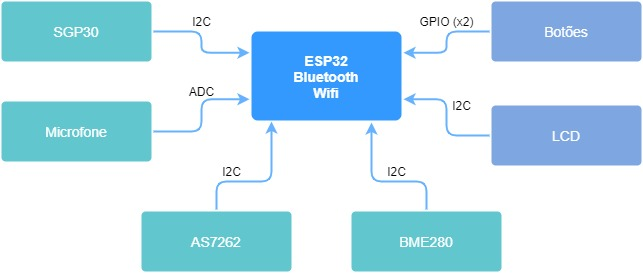
\includegraphics[width=12cm]{diagrama_hw_v1}
    \caption{Diagrama de Blocos de Hardware do Protótipo}
    \label{fig:img1}
\end{figure}

Quando possível, foram utilizados kits de desenvolvimento e módulos que nos permitisse uma validação mais rápida do hardware nessa fase inicial, permitindo avançar mais com o firmware e fazer testes em campo. 

O DevKitC do ESP32 possui integrado um USB, através do qual é possível alimentar os demais subcircuitos da placa, não existindo a necessidade de uso de bateria nessa etapa. 

\subsection{Esquemático}

Para o design do hardware, utilizamos o software de CAD de PCB \textit{Altium Designer 20} \cite{altium}. Foi utilizada a licença da empresa orientadora, sendo possível também conseguir uma licença gratuita para estudantes. Os arquivos estão disponíveis em \cite{git_hw}. 

A partir do diagrama de blocos, foi desenvolvido o esquema elétrico

\begin{figure}[h]
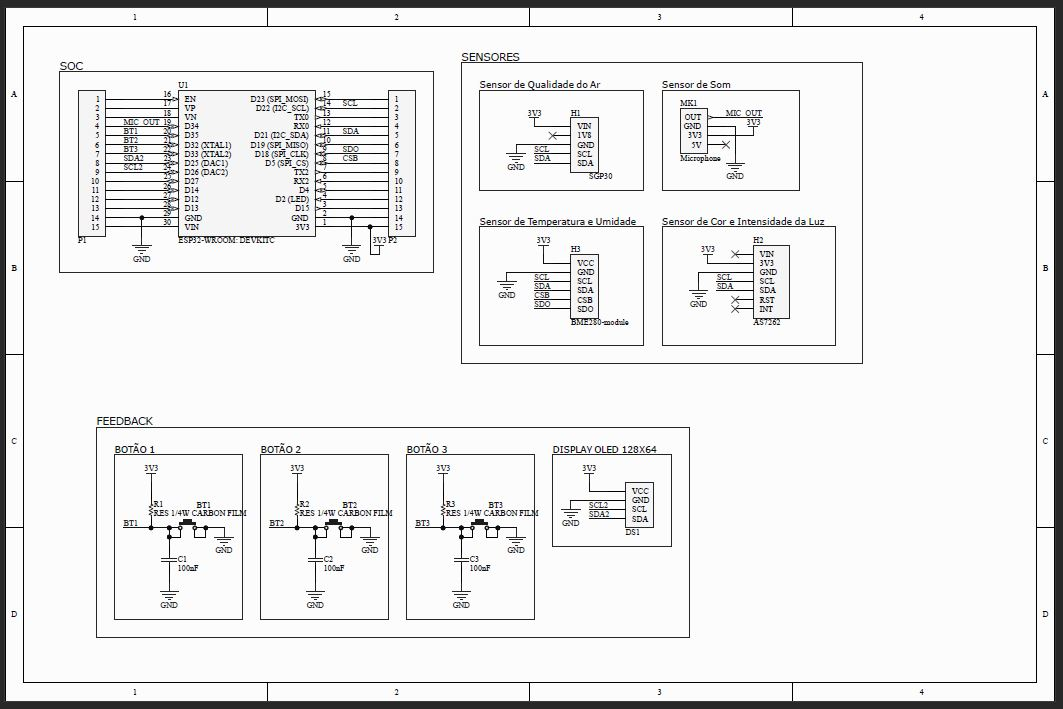
\includegraphics[width=\textwidth]{sch}
\caption{Esquemático do Protótipo}
\label{fig:img2}
\end{figure}

\subsection{PCB - \textit{Printed Circuit Board}}

A placa foi pensada como \textit{Single Layer}, para ser fabricada em fibra por uma fresadora CNC, com seus componentes e conectores soldados à mão. 

\begin{figure}[h]
\centering
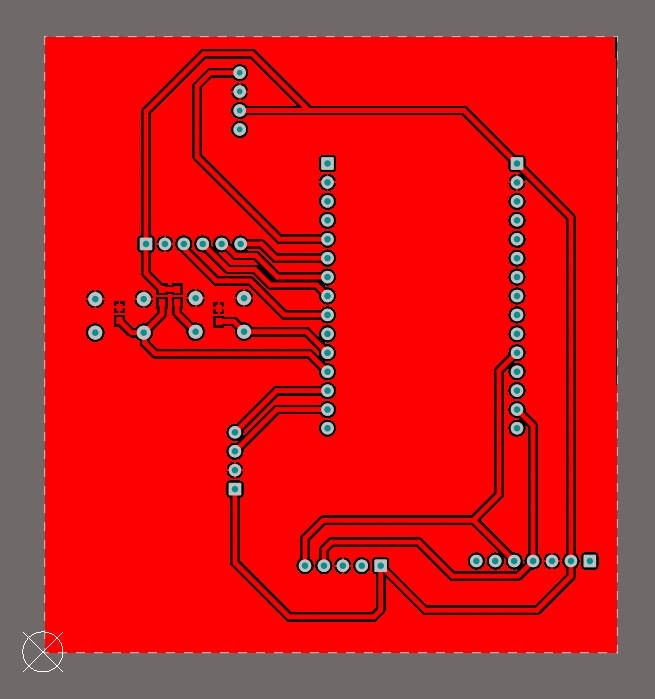
\includegraphics[width=8cm]{pcb_2}
\caption{Visão 2D da Camada Top Layer da PCB}
\label{fig:img3}
\end{figure}

\begin{figure}
\centering
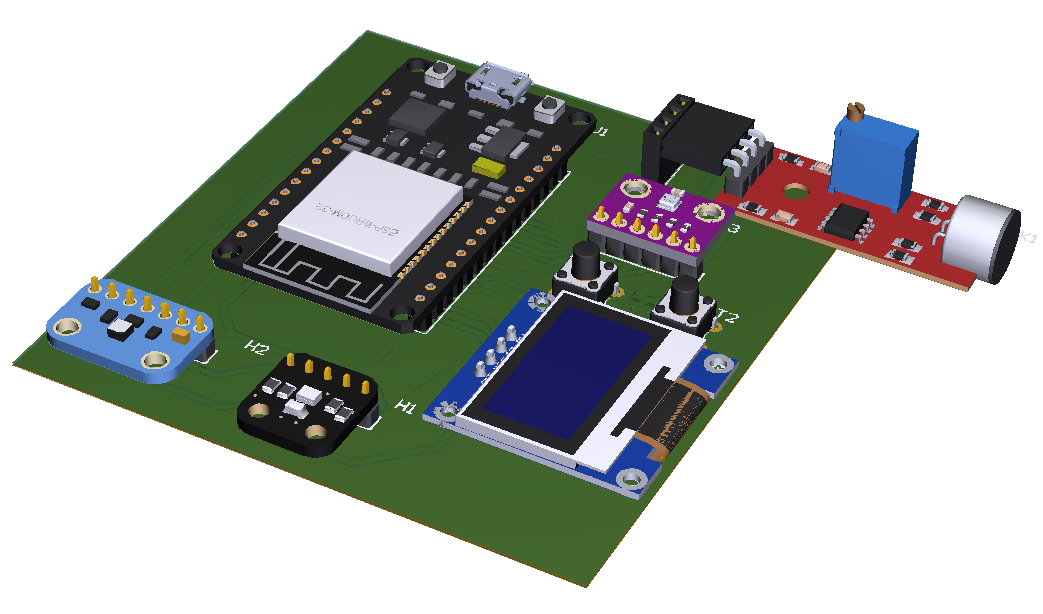
\includegraphics[width=10cm]{pcb}
\caption{Visão 3D da PCB}
\label{fig:img4}
\end{figure}

\section{Validação da Rede Mesh}


\end{document}